\subsection{Experimental setup}\label{subsec:experimental_setup}

\paragraph{Models and benchmarks.}
We use both base and instruct models of various scales, specifically Qwen2.5-Math-1.5B, Qwen2.5-Math-7B \citep{yang2024qwen25mathtechnicalreportmathematical}, Qwen2.5-7B \citep{qwen2025qwen25technicalreport} and LLaMA-3.1-8B-Instruct \citep{grattafiori2024llama3herdmodels}.
We consider three mathematical reasoning benchmarks: AIME 2024, AMC \citep{li2024numinamath}, and MATH-500 \citep{hendrycks2021measuring}.

\paragraph{Methods and evaluation.}
For test-time training, we use the VERL framework \citep{sheng2024hybridflow} with the GRPO algorithm \citep{shao2024deepseekmathpushinglimitsmathematical} on 8$\times$H100 Nvidia GPUs. We apply our method to each benchmark individually and report both pass@1 and majority-vote accuracy (see Appendix \ref{app:numerical_experiments_details}). We compare the performance of our proposed RL objectives with TTRL \citep{zuo2025ttrl}. 


\subsection{Results}\label{subsec:experimental_results}
Table \ref{tab:test-time-training-results} reports the pass@1 performance of various inference-time training strategies across different benchmarks and models. An extended version, comparing the improvements in pass@1 accuracy for both the score and format score, is provided in Table \ref{tab:test-time-training-results-pass1-format-score} (Appendix \ref{app:numerical_experiments_details}).
Overall, these strategies consistently enhance pass@1 performance, with the effect being particularly pronounced for Qwen2.5-Math-1.5B, the smallest model.
This suggest that such test-time methods help reveal the model’s underlying capabilities.


\begin{table}[t!]
\caption{Comparison of pass@1 performance before and after applying test-time training strategies.}
\vspace{-5pt}
\label{tab:test-time-training-results}
\begin{center}
\footnotesize
\begin{minipage}{0.47\linewidth}
\centering
\begin{tabular}{lccc}
\toprule
 & \textbf{AIME} & \textbf{AMC} & \textbf{Math\scriptsize-500\footnotesize} \\
\midrule
\textbf{Qwen2.5-7B} & 9.4 & 31.2 &  59.1 \\
SNR (Ours)& 23.3 &  51.8& 80.3 \\
Entropy (Ours)& 20.0 & 49.2 & 77.6 \\
\citet{zuo2025ttrl} & 24.3 & 53.4 & 79.6  \\
\midrule
\textbf{Llama-3.1-8B} & 4.4 & 21.8 & 48.2  \\
SNR (Ours)& 13.4 & 29.3 & 59.2 \\
Entropy (Ours)& 13.3 & 27.0  &  55.4 \\
\citet{zuo2025ttrl} & 10.0 & 32.3 & 63.7 \\
\bottomrule
\end{tabular}
\end{minipage}
\hfill
\begin{minipage}{0.47\linewidth}
\footnotesize
\centering
\begin{tabular}{lccc}
\toprule
 & \textbf{AIME} & \textbf{AMC} & \textbf{Math\scriptsize-500\footnotesize} \\
\midrule
\textbf{Qwen2.5-Math-7B} & 10.6 & 31.0 & 47.1\\
SNR (Ours) & 36.7 & 65.0 & 84.5 \\
Entropy (Ours) & 38.3 &  65.4 & 82.4 \\
\citet{zuo2025ttrl} & 37.9 & 63.5 &  83.6\\
\midrule
\textbf{Qwen2.5-Math-1.5B} & 7.1 & 28.1 & 31.4 \\
SNR (Ours)& 16.3  & 45.4 & 72.0 \\
Entropy (Ours)& 15.6  & 45.9 & 70.8 \\
\citet{zuo2025ttrl} & 15.8 & 48.4 & 71.9 \\
\bottomrule
\end{tabular}
\end{minipage}
\end{center}
\vspace{-10pt}
\end{table}
\normalsize




Besides, we analyse how test-time training reduces the number of samples required to guarantee, with high confidence, that the majority vote $\widehat{c}_n$  matches the true mode $c^\star$. 
Specifically, Table \ref{tab:stopping-rule-samples-results} reports the majority vote accuracy and the required number of samples under the MMC stopping rule $(N_{\text{adaptive}})$ for two confidence levels, $\varepsilon = 0.1$ and $0.4$, comparing the pre-trained model with the model after test-time training using SNR-based rewards. 
For reference, we also include the majority vote accuracy obtained when using the full sample budget $N_{\text{budget}}$.

We observe that the MMC adaptive sampling scheme substantially reduces the number of samples without causing a noticeable degradation in performance. Moreover, the number of samples required under the MMC stopping rule further decreases after applying test-time training, relative to the pre-trained model. 
This effect is examined in more detail in Table~\ref{tab:ratio_adaptive_sampling_pre_post_trained}, which reports the reduction in the ratio between $N_{\text{adaptive}}$ and $N_{\text{budget}}$ (given their approximately linear relationship). 
The decrease in this ratio after test-time training is most pronounced for the smaller 1.5B model.
Improving sample efficiency is particularly important, as it directly translates to lower inference costs.


Finally, since the MATH-500 dataset classifies questions into five levels of increasing difficulty, we analyse the distributions of the estimated lower bound of the probability $\mathbb{P}[\widehat{c}_n = c^\star]$, as well as the estimated signal-to-noise ratio $\reallywidehat{\text{SNR}}(\Delta_{j_n^\star})$ across these difficulty levels.
Figure~\ref{fig:violin_plots_main_text} shows that harder questions exhibit greater variability for both $\mathbb{P}[\widehat{c}_n = c^\star]$ and the SNR. 
In addition,  for the smaller 1.5B model, both the  probabilities and SNR distributions are more concentrated near zero for difficult questions compared to the 7B model.
These observations further support the idea that the SNR can serve as a label-free proxy for problem difficulty.




\begin{table}[t!]
\caption{Comparison of majority vote accuracy and required number of samples under the MMC stopping rule $(\mathbf{N}_{\text{adaptive}})$  for $\varepsilon = 0.1$ and $0.4$ between the pre-trained model and after test-time training with SNR-based rewards. Performance is compared to that obtained using the full sample budget ${N_{\text{budget}}}$ (\textcolor{red}{\xmark}). Results are shown for the MATH-500 dataset.}
\label{tab:stopping-rule-samples-results}
\begin{center}
\footnotesize
\begin{tabular}{lccccc}
\toprule
\multirow{3}{*}{$\mathbf{N_{\text{budget}}}$}& \multirow{3}{*}{\makecell{\textbf{Adaptive} \\ \textbf{sampling?}}} & \multicolumn{2}{c}{\textbf{Qwen2.5-Math-7B}}& \multicolumn{2}{c}{\textbf{Qwen2.5-Math-1.5B}}\\
\cmidrule{3-6}
& & \textbf{Pre-trained}& \textbf{Test-time trained} & \textbf{Pre-trained}& \textbf{Test-time trained}\\
& & \textbf{\%} \scriptsize$(\mathbf{N}_{\text{adaptive}})$& \textbf{\%} \scriptsize$(\mathbf{N}_{\text{adaptive}})$ & \textbf{\%} \scriptsize$(\mathbf{N}_{\text{adaptive}})$& \textbf{\%} \scriptsize$(\mathbf{N}_{\text{adaptive}})$\\
\midrule
\multirow{5}{*}{\textbf{10}} &\multirow{1}{*}{\textcolor{red}{\xmark}} &61.6&85.2&36.0 & 78.6\\
&\greencheck& \multirow{2}{*}{61.6 \scriptsize\textbf{(9.7)}}& \multirow{2}{*}{85.2 \scriptsize\textbf{(9.4)}}& \multirow{2}{*}{36.0 \scriptsize\textbf{(9.9)}} & \multirow{2}{*}{78.6 \scriptsize\textbf{(9.4)}}\\
& $\varepsilon = 0.1$&  &  & &\\
&\greencheck& \multirow{2}{*}{61.6 \scriptsize\textbf{(9.2)}}& \multirow{2}{*}{85.2 \scriptsize\textbf{(8.9)}}& \multirow{2}{*}{36.0 \scriptsize\textbf{(9.7)}} & \multirow{2}{*}{78.6 \scriptsize\textbf{(8.6)}}\\
& $\varepsilon = 0.4$& &  &  &\\
\midrule
\multirow{5}{*}{\textbf{50}} &\multirow{1}{*}{\textcolor{red}{\xmark}} & 62.2& 85.6& 37.6& 80.8\\
&\greencheck& \multirow{2}{*}{61.8 \scriptsize\textbf{(39.3)}}& \multirow{2}{*}{85.6 \scriptsize\textbf{(37.6)}}& \multirow{2}{*}{37.6 \scriptsize\textbf{(45.6)}} & \multirow{2}{*}{80.8 \scriptsize\textbf{(34.1)}}\\
& $\varepsilon = 0.1$&  &&  &\\
&\greencheck& \multirow{2}{*}{61.8 \scriptsize\textbf{(38.0)}}& \multirow{2}{*}{85.4 \scriptsize\textbf{(33.4)}}& \multirow{2}{*}{37.4 \scriptsize\textbf{(43.0)}} & \multirow{2}{*}{80.8 \scriptsize\textbf{(31.2)}}\\
& $\varepsilon = 0.4$&& & &\\
\midrule
\multirow{5}{*}{\textbf{100}} &\multirow{1}{*}{\textcolor{red}{\xmark}} & 62.2 & 85.6&\multirow{1}{*}{36.6} & 81.2\\
&\greencheck&  \multirow{2}{*}{62.2 \scriptsize\textbf{(74.9)}}& \multirow{2}{*}{85.6 \scriptsize\textbf{(67.2)}}& \multirow{2}{*}{36.8 \scriptsize\textbf{(86.5)}} &\multirow{2}{*}{81.0 \scriptsize\textbf{(61.2)}}\\
& $\varepsilon = 0.1$&  & &  &\\
&\greencheck& \multirow{2}{*}{62.2 \scriptsize\textbf{(73.1)}} & \multirow{2}{*}{85.4 \scriptsize\textbf{(60.8)}}& \multirow{2}{*}{36.4 \scriptsize\textbf{(81.8)}} &\multirow{2}{*}{80.8 \scriptsize\textbf{(56.9)}}  \\
& $\varepsilon = 0.4$& &  &  &\\
\bottomrule
\end{tabular}
\end{center}
\end{table}
\normalsize




\begin{figure}[h!]
  \centering
  \begin{subfigure}{0.49\textwidth}
      \centering
      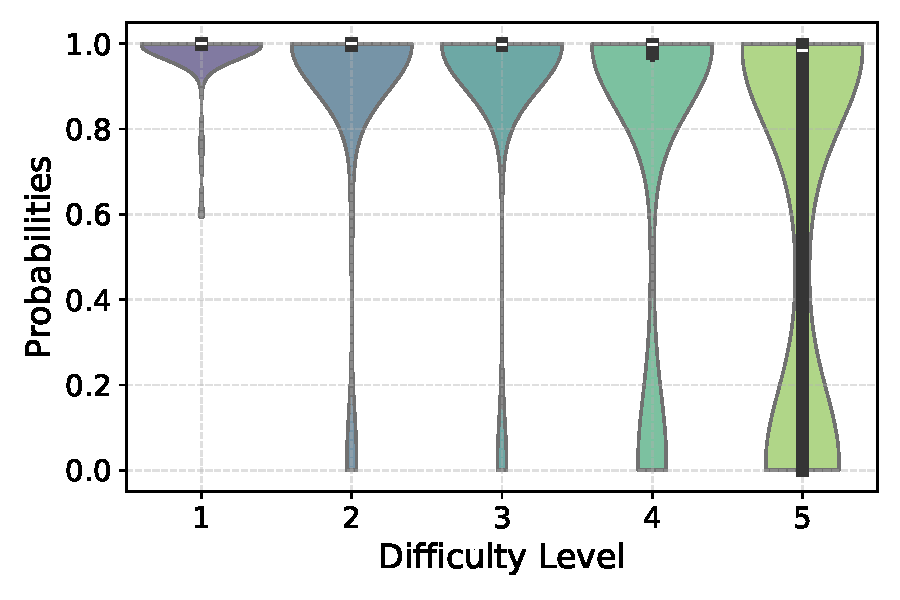
\includegraphics[width=\textwidth]{figs/QWEN-MATH-1.5B_violin_maj100_probability_adaptive_01_NO_ground_truth.pdf}
      \caption{Qwen2.5-Math-1.5B, $\mathbb{P}[\widehat{c}_n = c^\star]$.}
      \label{fig:QWEN-MATH-1.5B-probs-0.1}
  \end{subfigure}
  \hfill
  \begin{subfigure}{0.49\textwidth}
      \centering
      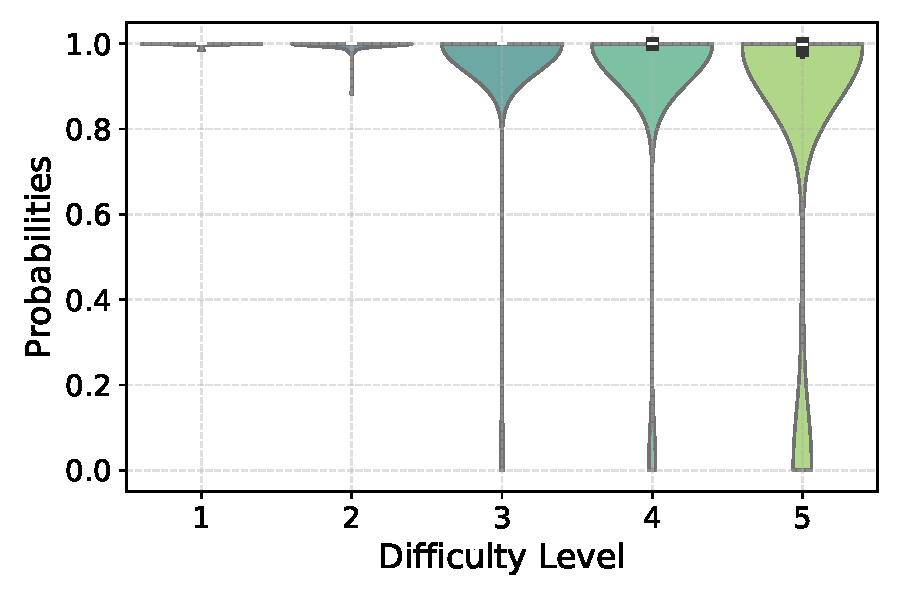
\includegraphics[width=\textwidth]{figs/QWEN-MATH-7B_violin_maj100_probability_adaptive_01_NO_ground_truth.pdf}
        \caption{Qwen2.5-Math-7B, $\mathbb{P}[\widehat{c}_n = c^\star]$.}
      \label{fig:QWEN-MATH-7B-probs-0.1}
  \end{subfigure}
  \vfill
  \begin{subfigure}{0.49\textwidth}
      \centering
      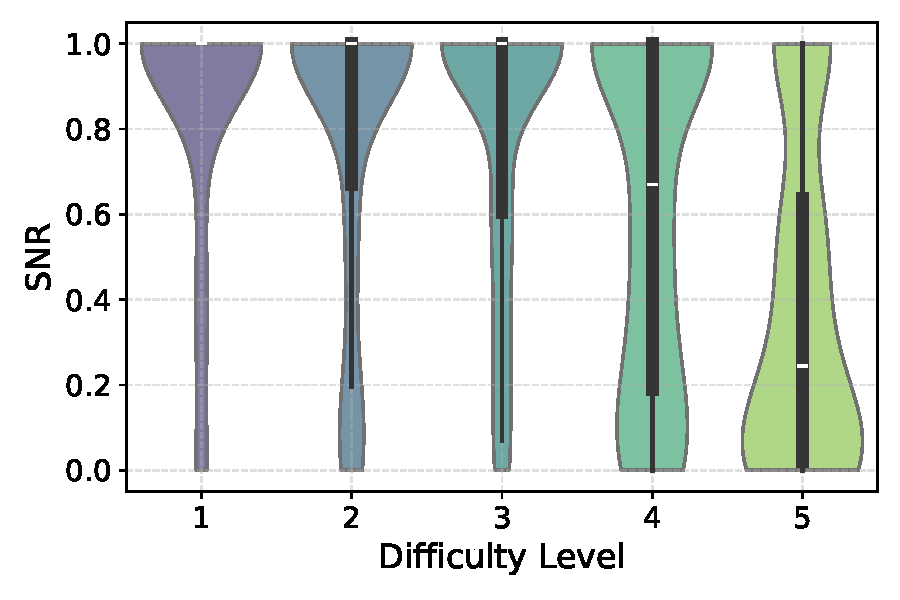
\includegraphics[width=\textwidth]{figs/QWEN-MATH-1.5B_violin_maj100_SNR_01.pdf}
      \caption{Qwen2.5-Math-1.5B, ${\text{SNR}}(\Delta_{j^\star_n})$.}
      \label{fig:QWEN-MATH-1.5B-SNR-0.1}
  \end{subfigure}
  \hfill
  \begin{subfigure}{0.49\textwidth}
      \centering
      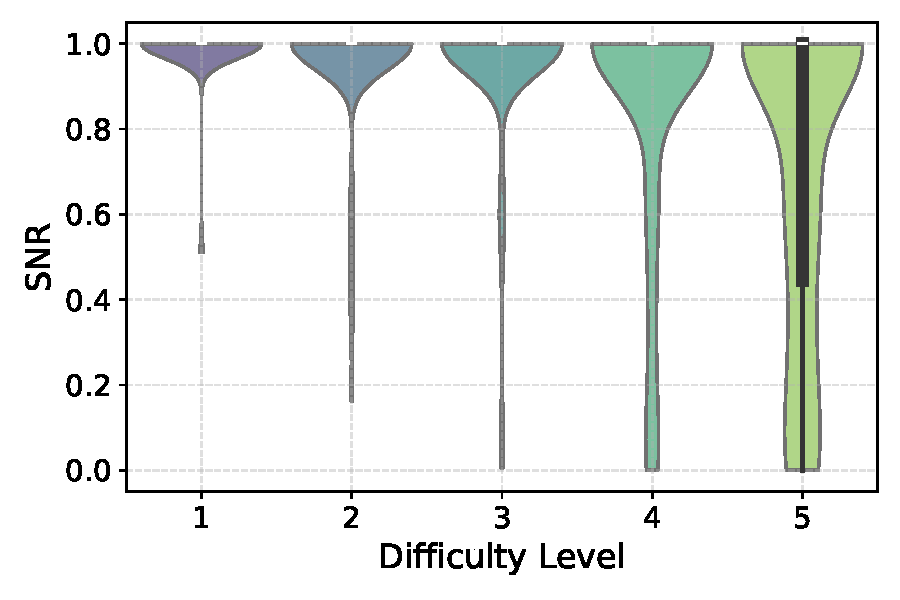
\includegraphics[width=\textwidth]
      {figs/QWEN-MATH-7B_violin_maj100_SNR_01.pdf}      
        \caption{Qwen2.5-Math-7B, ${\text{SNR}}(\Delta_{j^\star_n})$.}
      \label{fig:QWEN-MATH-7B-SNR-0.1}
  \end{subfigure}
  \caption{Distribution of the estimated lower bound of the probability $\mathbb{P}[\widehat{c}_n = c^\star]$ (computed via Beta approximations) and the signal-to-noise ratio $\text{SNR}(\Delta_{j^\star_n})$ when applying the MMC stopping rule with $\varepsilon = 0.1$ and $N_{\text{budget}}=100$. Results are obtained after test-time training with SNR-based rewards on the MATH-500 dataset.}
  \label{fig:violin_plots_main_text}
\end{figure}
